\documentclass[12pt,a4paper]{article}
\usepackage{graphicx}
\usepackage{biblatex}
\usepackage{parskip}
\usepackage{listings}
\usepackage{pdfpages}
\usepackage{rotating}
\usepackage{pdflscape}
\usepackage{amsmath}
\usepackage{subcaption} 

\lstset{%
basicstyle=\ttfamily,
breaklines = true,
tabsize=2
}
\graphicspath{ {./Images/} }
\addbibresource{biblography.bib}

\setlength{\parskip}{1em}
\begin{document}

\begin{titlepage}
	\newcommand{\HRule}{\rule{\linewidth}{0.5mm}}
    
\includegraphics[width = 4cm]{./Images/Logo.jpg}\\[0.5cm] 
    
    \center 
	\textsc{\large Department of Electrical and Electronic Engineering }\\[0.5cm] 
	\textsc{\normalsize ELEC40006: Electronics Design Project}\\[0.5cm] 
    
	\HRule \\[0.4cm]
	Circuit Simulator Technical Report
    \HRule \\[1.5cm]
     
    \begin{center}
		\underline{Authors}\\[0.5cm] Xin Wang\\CID: 01735253\\xin.wang19@imperial.ac.uk \\[0.5cm]
		Brandon Cann\\ CID: 01724765\\ brandon.cann19@imperial.ac.uk\\[0.5cm]
		Adam Rehman\\ CID: 01720256\\adam.rehman19@imperial.ac.uk\\[0.5cm]
	\end{center} \large
    
    \vfill % Fill the rest of the page with whitespace
 	\small Word Count: 4853 \\ [0.5cm]
    \makeatletter
    \@date 
    \makeatother
\end{titlepage}

\tableofcontents
\pagebreak

\section{Overview of the report}
Report layout loosely follows the stages of the Software Development Cycle. \par
Section 2 detailed the design problem presented and the program requirements at are necessary for a preliminary design 
to be established. \par
Section 3 provideed a summary of the program development timeline and the details related to project management,
format of meeting minutes used to how the responsibilities are distributed among the project team. \par
Section 4 discussed the preliminary designs the team had produced and the rationale behind some design choices the team had 
implemented. \par
Section 5 gave a comprehensive overview of the program design, the functions and flowcharts used during program 
development. \par 
Section 6 investigated the design constraints of the program, the accuracy of the results had produced and the speed of 
execution as the circuit size varied.\par
Section 7 discussed the major unforeseen problems encountered by the team over the course of the project and 
how the team attempted to mitigate that problem. \par
Section 8 discussed the possible improvements noted by the team that could mitigate concerns encountered
by the team. \par
Section 9 detailed the possible features that can be added on to the existing program and the required modifications to the
program to add the mentioned features. \par 
Section 10 contained the reflections written by each teammate towards the end of the project. \par
\pagebreak

\section{Project Specification}
	\subsection{Design Problem}
	Develop a program that is able to read in a file describing a circuit specified by the user, perform 
	transient simulation on that circuit and output the calculated voltages at each instance in time into a specific file
	format. 
	\subsection{Program Requirements}
	The main program requirements are listed as follows:
	\begin{itemize}
		\item Program must support basic circuit components listed as follows \footnote{Advanced component can be supported
		provided basic components are already implemented.}:
		\begin{itemize}
			\item Resistors
			\item Ideal Capacitors
			\item Ideal Inductors
		\end{itemize}
		\item Parser to be designed to take in a input file of SPICE netlist format.
		\begin{itemize}
			\item Basic syntax checks to be performed.
		\end{itemize}
		\item The output file must be in Comma Separated Value (.CSV) format.
		\begin{itemize}
			\item Columns of output file represent nodes in the circuit.
			\item Rows of output file represent an instance in the simulation.
		\end{itemize}
	\end{itemize}
	\vfill
	\pagebreak
	\subsection{Design Criteria}
	The team had identified several factors from the list of factors given in the Product Design Specification
	\footnote{Document included in \textit{documents} folder.} document.
	\begin{itemize}
		\item Maintenance: One of the most important factors the team identified. As the development timescale was 
		constrained and the features required was open-ended, so it was very important we ensured the design could 
		incorporate new features efficiently and cost-effectively if the client wished to add new features.
		\item Documentation: For a non-intuitive program, proper documentation was required for client and future
		programmers to make modifications should the client wished.
		\item Performance: No strict performance guidelines are given by the client but the execution 
		speed should still be reasonable. 
		\item Time scale: 6 weeks with a definite deadline. It was important to balance proper team management
		techniques and creating a program that met client standards.
		\item Testing: Test programs have been created to test various aspects of the program to ensure
		accurate results have been produced. The results produced have been verified with LTSpice, a well
		established circuit simulation program.
		\item Patents: SPICE engine is a public domain software so we could possibly incorporate SPICE into 
		developing the program.
		\item Ergonomics: A Graphics User Interface (GUI) was not required by the client but it could possibly 
		make the program much easier to use.
	\end{itemize}
	\vfill
	\pagebreak

\section{Team Management}
	\subsection{Project timeline overview}
	Xin Wang managed the team's project timeline and any modifications to the timeline required the agreement of all
	teammates. \par
	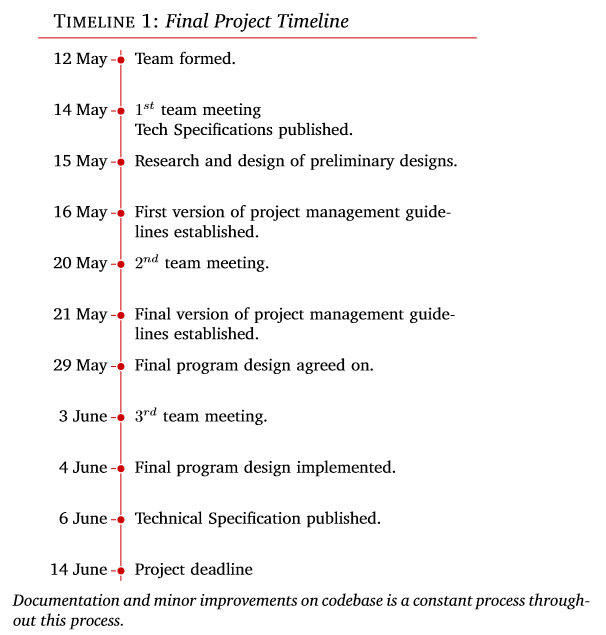
\includegraphics{Timeline.PNG}
	\pagebreak

	\subsection{Team Gnatt chart}
	The team Gnatt Chart waas created by using \textit{GnattProject} software. It was not the most 
	visually appealing software but, for its free features, it met the requirements of the team. \par
	The Gnatt Project was mainly modified by Xin Wang upon requests by teammates after team meetings. Please
	refer to Appendix: Gnatt Chart for details of the team's Gnatt Chart. \par
	\subsubsection{Important Notes:}
	\begin{itemize}
		\item Activities like ensuring standardised coding comments and formatting which had been monitored by 
		Xin Wang was a constant background activity. 
		\item A team meeting ocurred after each major stage of the Gnatt Chart finished (Indicated by 
		a change in colour).
		\item On the 5th June of 2020, Xin Wang received a notification for a repatriation flight
		and, in the following team meeting, the team agreed on redistributing Xin Wang's responsibilities
		and for him to finish the existing Technical Report.
	\end{itemize}
	\pagebreak

	\subsection{Management approach}
	The project team, after research on forms of project management, decided on using a Waterfall project
	management approach. The phases of the project are listed as follows: \par
	\begin{itemize}
		\item System and Software Requirements.
		\item Analysis.
		\item Design.
		\item Coding.
		\item Testing.
	\end{itemize}
	This method was selected mainly due to the short duration of the project, requirements are clear and the team 
	was not constantly required to report to the client at the early stages of the software development to ensure 
	client satisfaction. \par

	The Waterfall methodology prioritised proper documentation throughout the whole development process. This was important
	to the team as the team project required a Project Report to be submitted and, due to the ongoing remote lab orals and 
	family-related obligations during quarantine, allowed a team member to be quickly caught up if a member stepped out
	of the team for a while.  

	The disadvantage of the Waterfall methodology was mainly in that no working software was produced until late in the 
	cycle so there had been a level of risk and uncertainty with not being able to meet the deadline, especially in the 
	with the remote working environment \footnote{Any unforeseen circumstances are listed in team meeting minutes 
	summarised under the Critical Analysis section.}. 
	The team had later realised the methodology was not exactly suitable for the Object Orientated Approach 
	that the team wanted to implement. As the integration was done at the end, there was concerns in the possibility that any errors
	in the program would not be noticed during the integration stage.

	\vfill
	\pagebreak

	\subsection{Team responsibilities breakdown}
	The responsibilities of each team member was discussed during the 1st meeting and had been formalised in the 2nd meeting. The
	respective roles are influenced by the Belbin questionnaire provided.
	\footnote{Belbin questionnaire forms are found in Appendix: Belbin Roles.}
	\par
	The main responsibilities of each team member are listed as follows:
	\begin{itemize}
		\item Adam Rehman
		\begin{itemize}
			\item Belbin role: Plant
			\begin{itemize}
				\item Research program.
				\item Coding the program.
				\item Testing program.
			\end{itemize}
		\end{itemize}
		\item Belbin role: Brandon Cann
		\begin{itemize}
			\item Monitor Evaluator
			\begin{itemize}
				\item Ensure documentation managed by Xin Wang and coding managed by Adam was in sync.
				\item Contributes to program aspects that are falling behind.
				\item Ensure project requirements are met.
			\end{itemize}
		\end{itemize}
		\item Belbin role: Xin Wang
		\begin{itemize}
			\item Implementer
			\begin{itemize}
				\item Creating and managing the team Project Report and various other documentations.
				\item Meeting minute keeper.
				\item Ensuring code written was up to a standard format with proper comments.
				\item Manages repository base.
			\end{itemize}
		\end{itemize}
	\end{itemize}

	\vfill
	\pagebreak

	\subsection{Project meeting minutes}
	The meeting minutes follow a standard template that was attached under Appendix: Meeting Minutes. \par
	There was no standard protocol for calling team meetings, they are called usually when there was a problem
	that had affected all team members. Usually, there were smaller informal meetings across various channels from 
	WhatsApp to Discord. \par
	Over the course of the development cycle, there had been three formal meetings and the main reasons and conclusions
	are listed below.
	\begin{itemize}
		\item Meeting 1
		\begin{itemize}
			\item Reason: 
			\begin{itemize}
				\item Project team meeting each other. Not every team member knows each other.
				\item Discussed the Circuit Simulator Briefing.
			\end{itemize}
			\item Conclusions:
			\begin{itemize}
				\item Xin Wang was assigned as documentation manager and tasked with formalising the Project Requirement.
			\end{itemize}
		\end{itemize}
		\item Meeting 2
		\begin{itemize}
			\item Reason:
			\begin{itemize}
				\item With a draft of the project management guidelines, team discussed the team dynamics.
				\item Discussed general direction of our program design.
			\end{itemize}
			\item Conclusion:
			\begin{itemize}
				\item Agreed that practicing proper team management was just as important as showing practical skills 
				in coding.
				\item Final team management guidelines are agreed and tasked to Xin Wang to formalise in documentation.
			\end{itemize}
		\end{itemize}
		\item Meeting 3
		\begin{itemize}
			\item Reason:
			\begin{itemize}
				\item Program basic requirements are nearly fulfilled. 
				\item Meeting to discuss future program design direction.
				\item Xin Wang had a notification by South African Embassy of a Repatriation flight.
			\end{itemize}
			\item Conclusion:
			\begin{itemize}
				\item Plans set to divide up Xin's responsibilities among the other two team members.
				\item Documentation finalised and notes written by Xin passed to team members.
			\end{itemize}
		\end{itemize}
	\end{itemize}
	\pagebreak

	

\section{Preliminary Designs}
The initial program design relied on the project briefing provided. Parsing a input file into a data 
structure was a simple task. The main point of discussion was related to how the program solved for unknown voltages.
\par
The main design choices taken by the team has been set out below.
	\subsection{Object Orientated Programming [OOP]}
	As the circuit components the program needed to support was an open ended requirement except the mandatory basic components 
	listed, the team was concerned on the expandability of the program.
	\par
	The OOP approach allowed the program design to be rapidly and cost-effectively altered to accommodate new features
	such as new circuit components or analysis techniques \cite{OOP} that the client might request later on in the 
	program's lifecycle. Increased program maintainability will save the programmer time and the client cost in program's 
	active lifetime.
	\par
	The disadvantage was that it has been shown to be slower than other preliminary programs designed 
	without OOP to an average of of 5\% to 10\% slower depending on other optimisations in the program.
	\par 
	It was the team's view that execution speed was not the highest priority and the ability to expand the program's feature set
	was also important. The design was detailed in the next section.

	\subsection{Modified Nodal Analysis}
	Modified Nodal Analysis (MNA) was an extension of normal Nodal Analysis. When the team studied similar 
	programs like PSPICE and LTSpice, MNA had been mentioned numerous times \cite{MNA} and its benefits had been proved during
	trails of programs based on preliminary designs. A problem the team encountered was trying to 
	represent the current-dependent circuit elements like inductors efficiently. 
	\par
	As stated earlier, it was a primary concern of the team the scalability of the program. By using MNA, just like
	other commercial programs, the team was confident that the analysis component of the program would not be a 
	bottleneck to future developments of the program.
	\par
	The advantage of MNA was in its standard procedures. The standardised MNA algorithm for solving nodal 
	equations allowed the team to modularise the solving aspect of the program. This meant not constantly be required to 
	make changes to one of the most important parts of the program, instead just ensuring the component was in the 
	compatible format to be entered into the MNA algorithm.
	\par 
	The MNA algorithm consisted of three matrices that form the matrix relation: $Ax=b$ \cite{MNA}:
	\begin{itemize}
		\item $A$ was consisted of four sub-matrices which included the admittance matrix. The program treated matrix $A$ as 
		a whole matrix instead of four smaller matrices and combining at the end.
		$$ A =
		\begin{bmatrix}
			G & B\\
			C & D 
		\end{bmatrix} $$

		\item $x$ represented the unknown node voltages and current of the voltage sources.
		$$ x =
		\begin{bmatrix}
			v \\
			i_{v} 
		\end{bmatrix} $$

		\item $b$ contained the values of voltage sources and current sources in the circuit.
		$$ b =
		\begin{bmatrix}
			i \\
			e 
		\end{bmatrix} $$

	\end{itemize}
	The admittance matrix was created during initialisation stage of the simulation. Non-linear elements are converted into 
	suitable formats at each instance in time during transient simulation. The resulting model parameters are 'stamped' into the matrix
	at each instance. Only 'stamping' the changing values instead of creating a new system of matrices saved valuable execution time
	during program execution. The matrix inversion was handled by the Eigen library, the library supported various types of 
	inversion with different accuracy and speed, this was discussed under the Optimisation sector.

	\subsection{Eigen Matrix Library}
	In terms of matrix operations, the team had decided to use a third-party program to handle the matrix-related operations in
	order to save development time and minimise potential errors.
	The primary concern the choice of third-party program was how seamless the program integrated into our program. 
	The team did not know whether the client would be comfortable installing an unknown third-party program on their system 
	besides the program the client specifically requested.\par
	There are third-party programs that required installation such as Armadillo and some had a large file size such as the 
	Boost Library which was close to 1GB.
	Based on the concerns laid out, the team looked for a program that has a reasonable size, does not require installation 
	in order to be used. The third-party program chosen was Eigen. It was a file that had a reasonable size and only required that the
	Eigen library was located in the same directory. A copy of Eigen was included in the program files for client's ease of usage.
	\pagebreak

\section{Program Design}
	\subsection{Top level view of the program}
	\begin{figure} [h!]
		\centering
		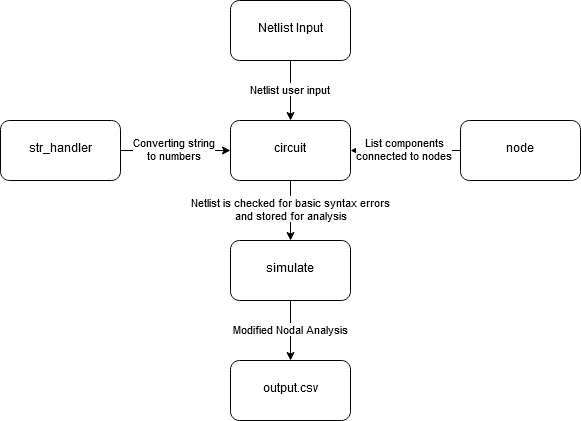
\includegraphics[scale=0.5]{Flow chart.PNG}
		\caption{General flowchart of program}
	\end{figure}
	\textit{circuit.hpp} file formed the centre of the program, handled the input of the file and 
	stored it in a form that allowed the \textit{simulate} file to perform Transient Analysis on it and output
	the file in the format (.CSV) specified by the client.
	\par
	The theoretical information and program design for each of the main files are discussed in the following 
	sections.
	\pagebreak
	\subsection{Components files}
	Due to the OOP design methodology, each component and its necessary functions are described in its own
	respective file. The file \textit{edge.hpp} is the base from which all other circuit components are derived
	from the \textbf{components} folder. 
	\subsection{\textit{str handler.hpp} file}
	The \textit{str handler} file managed all string-related functions. \par
	The main function is the \textit{tokenisier} function which take in an 
	input sentence and separated it into individual words that can be processed, 
	converted into the required formats for processing and storage. \par
	During conversions, checks are performed at various stages. In the product briefing, there
	was no mention of error handling requirements but the team viewed that defensive programming 
	was required and any errors encountered will be displayed to the user. 

	\subsection{\textit{node.hpp} file}
	A circuit can be expressed as a Network Graph, containing branches and edges. This notation was used to abstractly express
	the circuit and arrange how the the program operates.
	The function of the \textit{node.hpp} file is to represent a node in the circuit and allow nodal equations
	to be created.\par
	This function was not necessary in the final design as the program skipped creating nodal
	equations and directly input entries into the matrix before solving it. This part is kept to allow other functions to 
	be developed such as printing nodal equations.
	\pagebreak
	\subsection{\textit{circuit.hpp}}
	As mentioned previously, \textit{circuit.hpp} managed all aspects of the program from 
	reading in the user input, checking basic syntax errors during user entry 
	to ensuring the simulation is successful.
	Numerous checks are performed over the course of the simulation and any errors encountered
	will instantly result in the simulation ending with an error message outputted. \par
	
	The flow chart of \textit{circuit.hpp} is shown as below: \par
	\begin{figure} [h!]
		\centering
		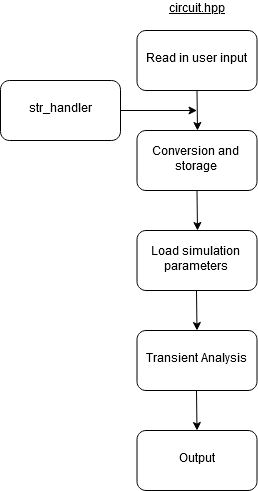
\includegraphics[scale=0.5]{circuit.PNG}
		\caption{Circuit flow chart}
	\end{figure}
	\pagebreak
	\subsection{\textit{simulate.hpp}}
	This section of the program was where the team has spent most of the time and also where the
	team saw many possible optimisations which will be discussed in later sections. This 
	section handled matrix entry and controlled the transient simulation. \par
	But using the MNA technique, basic components such as voltage sources, current 
	sources and resistors are simple and can be directly entered into the matrices for 
	solving. However, components such as inductors and capacitors which are non-linear
	devices required further processing in order to support those components. 
	At each instance in time, non-linear components need to be approximated into corresponding
	companion models. With the program using MNA, all non-linear components are converted 
	into a current source and resistor to allow efficient entry into the matrix.
	\subsubsection{Non-linear components}
	In the process of approximating non-linear components, integration would be 
	required and there are three different 
	methods of integration each with its own corresponding equations defining 
	current and resistance of the companion model. Each type of integration offers different
	degrees of accuracy which are explored under the Optimisation section.\par
	Capacitors are defined with the following differential equation:
	$$I=C\times \frac{dv}{dt}$$
	Inductors are defined with the following differential equation:
	$$V=L\times \frac{di}{dt}$$
	
	\begin{figure} 
		\centering
		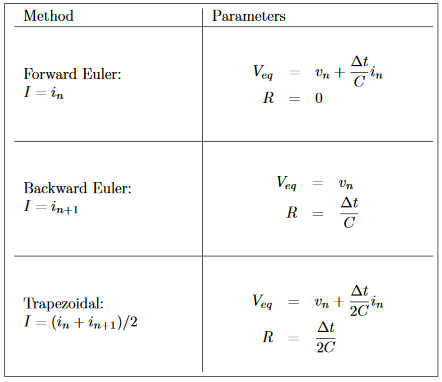
\includegraphics[scale=0.90]{capacitor.PNG}
		\caption{\centering Capacitor companion model parameters for different types of integration 
		\cite{companion}}
	\end{figure} 
	\begin{figure} 
		\centering
		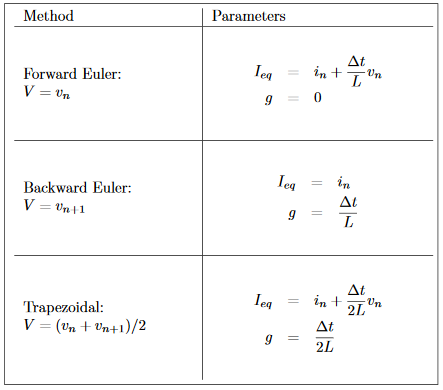
\includegraphics[scale=0.90]{inductor.PNG}
		\caption{\centering Inductor companion model parameters for different types of integration 
		\cite{companion}}
	\end{figure}
	\pagebreak
	\subsubsection{Simulation flowchart} 
	The listed simulation flowchart has not accounted for approximating components like Diodes which need Newton-Raphson 
	iteration.
	\begin{figure} [h!]
		\centering
		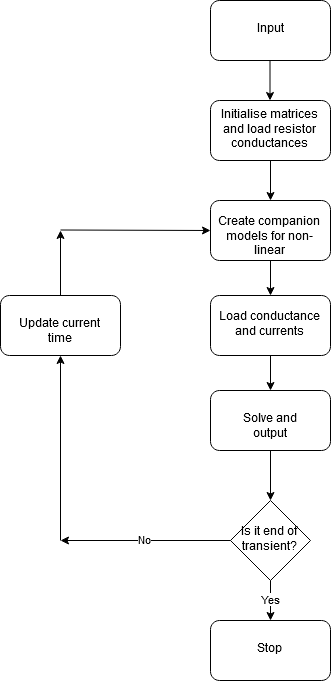
\includegraphics[scale=0.5]{simulate.PNG} 
	\end{figure} 
\pagebreak

\section{Testing}
It should be noted that majority of the testing was done on Linux Ubuntu 16.04.1 LTS which ran on a virtual machine in Windows 10,
some testing have been completed on a Windows 10 machine. As such, the listed execution times are the average of 10 execution
times. \par 
Numerous functions are imbedded into the program itself to aide the benchmarking process and can be used to aide in debugging.
\pagebreak
\section{Critical Analysis}
Throughout the process of program development, the team encountered two unforeseen circumstances that set the team back 
and required some adjustments on the timeline.
\subsection{OOP design}
It was felt strongly by the team that OOP design was required by the program. However, how the modules of the program were 
arranged was a topic that was argued and constantly revised. \par 
To this problem, the team researched articles that investigated how circuit simulators could be implemented from the 
OOP perspective and, also, the team drew inspirations from the technical documentations of more established circuit 
simulation programs like SPICE3 and PSpice.
\subsection{Repatriation Flight}
On the 4th of June 2020, Xin Wang received a notification of a possible repatriation flight for South African citizens.
As the exact time of the flight is not known yet and there was no guarantee that the quarantine site would have WIFI, it
was very likely that Xin Wang could not be reached once arriving at South Africa. There was many unknown variables and the 
responsibilities that Xin Wang handled was very critical in this final stage of the program. \par 

In the final team meeting, the team was briefed by Xin Wang of the state of the reports and what was still outstanding. 
As it was the weekend, the team could not reach the professors in charge of the project so the team had to make the 
decisions, mitigate the possible effects of Xin's absence and seek guidance as soon as possible.
The steps the team undertook are summarised as below:
\begin{itemize}
	\item Xin Wang to complete what can be completed on the report (Some data such as Testing has been completed yet)
	\item Xin Wang, once report is completed, shall handover the responsibilities to the remaining two teammates.
	\item Xin Wang will document any ideas he has yet to implement such as a guide to the demo video talking points.
	\item Tasks that the two teammates still have to complete:
	\begin{itemize}
		\item Advanced component support
		\item Demo video
		\item Testing results and report  
	\end{itemize}
\end{itemize}
The team understood that in the workplace, there would be unforeseen circumstances that affected the team's workflow.
It was important that the client's basic requirements are still met albeit some of the more advanced features would not be 
able to be completed but will still be documented under section: Adding On for the client to see and consider implementing.
\par 
Xin Wang will constantly keep the team brief on whether he can lend any help in preparing the program for submission. However
in order to minimise unknown variables, the team planned with the possibility of Xin Wang not being able to communicate and the
remaining team will have to handle report submission and video demonstration.
\pagebreak
\section{Optimisations}
\subsection{Sparse Matrices}
Various circuit simulation engines like SPICE uses sparse matrices and it was mentioned \cite{OOP} during our research stage but 
the current program used dense matrices. The primary concern was stability of the program as the team did not have 
any experience with Sparse Matrices but the Eigen Library is able to implement sparse matrices. \par
With the current supported circuit components, using dense matrices does not affect the program speed significantly. But as 
the circuit size gets bigger and more complicated components like operational amplifiers is supported, the matrices would
get bigger. The memory used and the processing power used would increase proportionally. \par
Sparse matrices solves that problem as numerous entries of the matrices is zero and does not affect the results. The benefit is
reduced memory usage and much faster program execution times which is a bottleneck in the current design.
Due to the OOP program design, it can be quickly implemented but extensive testing would be needed.
\subsection{Integration method}
There are numerous different types of integration but the three most common forms of integration are as follows:
\begin{itemize}
	\item Forward Euler
	\item Backward Euler
	\item Trapezoid
\end{itemize}
Out of the three, Trapezoid was the most accurate form of integration but the most processor intensive form of integration listed.
The report had listed the three forms of integration and its respectively defined parameters. 

\begin{figure} [h!]
	\centering
	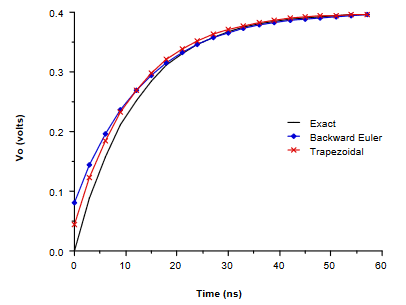
\includegraphics[]{Integration.PNG}
	\caption{Accuracy comparison of different integration methods \cite{integration}}
\end{figure}
\par
But Euler's methods are only accurate to the first degree and Trapezoid to the second degree.
Other methods such as the Runge-Kutta method would be much more accurate.
This method would rely on creating a specialised function that exclusively handles it and would add to the processing time but,
if sparse matrices were implemented, the team believes it would still result in a faster program.

\subsection{Inversion method}
The Eigen library supported numerous types of equation solver functions. The default type that the Eigen documentation support was the 
\textit{ColPivHouseholderQR} method but, using it, resulted in a average execution time of 50\% longer. Instead, the team 
did not use the equation solver functions. The team used the inversion function on matrix $A$ and multiplied it directly to matrix $b$.
\par 
The team believes that there would be more efficient third-party algorithms that can help make the program more efficient. For example, 
the Boost Library contains numerous functions that can entirely eliminate the need for the \textit{str handler.hpp} file and,
as it is a extensively supported library, it would be more efficient to use it. But it would require client consultations to ensure
the client understands and was comfortable with a larger program size. 
\pagebreak

\section{Adding on}
\subsection{Graphics User Interface}
The current user interface was very limited, it consisted of only a basic interface created
with bash script. The output file, though in .CSV format, required the user to 
use third-party programs like MatLab to plot the graph. If the user used the third-party
program, GNUPLOT, it was possible to integrate graph plotting feature directly into the existing 
script. 
\par 
Alternatively, a more user intuitive interface can be created in the future. Given the 
limited programming capability of the team, a third-party program to support the 
development of the User Interface is seen as the most viable by the team. Through research, the 
team has identified several possible programs that could be used:
\begin{itemize}
	\item \textit{Qt}
	\item \textit{wxWidgets}
	\item \textit{gtkmm}
\end{itemize}
The team's primary research is centered on the \textit{Qt} program. \textit{Qt} is a open
source program and it is relatively easy given its complete feature set, using that program
would minimise development cost and the interface features would not be limited.

Furthermore, with the C++ programming language used to create the program and the compatibility
of \textit{Qt} with C++, the team feels confident Qt would be the program used by the team
to implemented the Graphical User Interface.

\subsection{Components supports}
\subsubsection{Diode}
For non-linear components like the Diode, a function would need to be created that will be able to 
approximate the component into a compatible model for our program. The diode is defined by the 
following relation $$i(v)=I_s(e^{(\frac{v}{V_t})}-1)$$

By using the Newton-Raphson method, the non-linear equation is linearised to the following equation\cite{companion}
$$i_{lin} = (i(v_n)-gv_n) + gv$$
The equation can then be used to derive the following companion model:

\begin{figure} [h!]
	\centering
	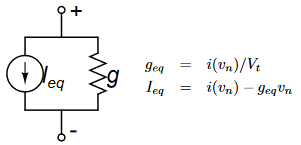
\includegraphics[]{diode_model.PNG}
	\caption{Companion model of the diode and its defining parameters \cite{companion}}
\end{figure}
As the Newton-Raphson iteration method requires the calculations to converge to a solution, in the event that it does not
converge and max repetitions have been reached, the program could implement a convergence helper such as \textit{gMin stepping} or
\textit{source stepping} and, if there is no more convergence helpers left, then the program will output an error to the user.
The process of Newton-Raphson has many 
possible optimisations to improve the convergence such as improving the model used and the algorithm of the existing model.
\par 
The basic convergence parameters that would govern whether convergence has been met will be defined as:
\begin{itemize}
	\item RELTOL: Tolerance of voltages and currents.
	\item VNTOL: Tolerance of nodal voltages.
	\item ABSTOL: Tolerance of branch current.
	\item ITL: Max number of iterations allowed.
\end{itemize} 
The existing program flow chart would have to be modified to accommodate the Newton-Raphson iteration method. 
\begin{figure}
	\centering
	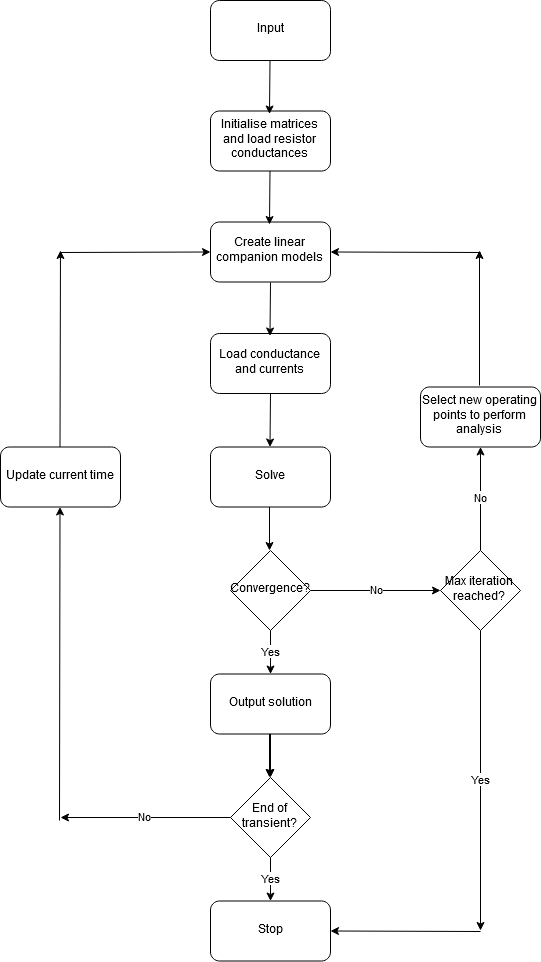
\includegraphics[scale=0.5]{Newton_Raphson.png}
	\caption{Program Flowchart incorporating Newton-Raphson method}
\end{figure}

\pagebreak
\subsubsection{Voltage controlled voltage sources - VCVS}
VCVS would be defined in the netlist in the following format: \par 
\begin{figure} [h!]
	\centering
	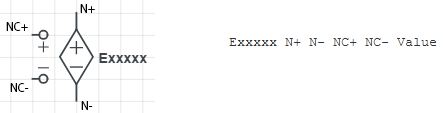
\includegraphics[]{E.png}
	\caption{Netlist format describing a VCVS \cite{MNA}}
\end{figure}
The output voltage of a VCVS is defined by the following equation: $$V_{out}=Value \times (V_{NC+}-V_{NC-})$$
where $V_{NC+}$ and $V_{NC-}$ are the controlling nodes. Due to the MNA method used by the program, supporting VCVS is 
easily done by modifying the existing system of matrices and solving for unknowns.

\begin{figure} [h!]
	\centering
	\begin{subfigure}{.5\textwidth}
	  \centering
	  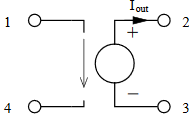
\includegraphics[scale=0.8]{E_diagram.PNG}
	  \caption{Circuit symbol of a VCVS}
	  \label{fig:sub1}
	\end{subfigure}%
	\begin{subfigure}{.5\textwidth}
	  \centering
	  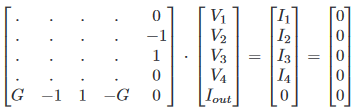
\includegraphics[width= \textwidth]{E_matrices.PNG}
	  \caption{MNA matrix entry}
	  \label{fig:sub2}
	\end{subfigure}
	\caption{MNA matrix for a VCVS \cite{jahn_margraf_habchi_jacob_2003}}
	\label{fig:test}
\end{figure}

\subsubsection{Voltage controlled current sources - VCCS}
VCCS would be  defined in the netlist in the following format: \par 
\begin{figure} [h!]
	\centering
	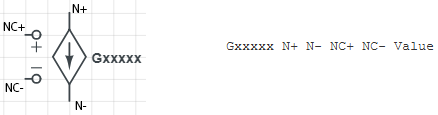
\includegraphics[]{G.png}
	\caption{Netlist format describing a VCCS \cite{MNA}}
\end{figure}
VCCS output is considered as a current source hence only introduce one more unknown into the MNA matrix. 
It could be defined as the following:
\begin{figure} [h!]
	\centering
	\begin{subfigure}{.5\textwidth}
	  \centering
	  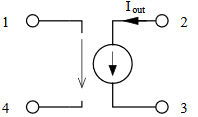
\includegraphics[scale=0.8]{G_diagram.PNG}
	  \caption{Circuit symbol of a VCCS}
	  \label{fig:sub1}
	\end{subfigure}%
	\begin{subfigure}{.5\textwidth}
	  \centering
	  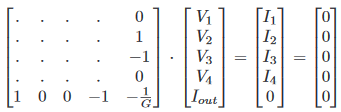
\includegraphics[width= \textwidth]{G_matrices.PNG}
	  \caption{MNA matrix entry}
	  \label{fig:sub2}
	\end{subfigure}
	\caption{MNA matrix for a VCCS \cite{jahn_margraf_habchi_jacob_2003}}
	\label{fig:test}
\end{figure} \pagebreak

\subsubsection{Current controlled voltage sources - CCVS}
CCVS would be defined in the netlist in the following format: \par
\begin{figure} [h!]
	\centering
	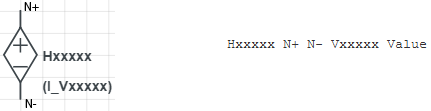
\includegraphics[]{H.png}
	\caption{Netlist format describing a CCVS \cite{MNA}}
\end{figure}

The controlling variable is current through one of the voltage sources listed as the controlling element in the netlist.
As MNA also calculates the current through the voltage sources, it will be relatively simple to extract that current
value and find the output of the CCVS. CCVS creates two more unknown variables.
It could be defined as the following:
\begin{figure} [h!]
	\centering
	\begin{subfigure}{.5\textwidth}
	  \centering
	  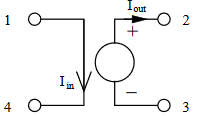
\includegraphics[scale=0.8]{H_diagram.PNG}
	  \caption{Circuit symbol of a CCVS}
	  \label{fig:sub1}
	\end{subfigure}%
	\begin{subfigure}{.5\textwidth}
	  \centering
	  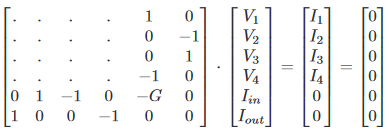
\includegraphics[width= \textwidth]{H_matrices.PNG}
	  \caption{MNA matrix entry}
	  \label{fig:sub2}
	\end{subfigure}
	\caption{MNA matrix for a CCVS \cite{jahn_margraf_habchi_jacob_2003}}
	\label{fig:test}
\end{figure}
\pagebreak
\subsubsection{Current controlled current sources - CCCS}
CCCS would be defined in the netlist in the following format: \par
\begin{figure} [h!]
	\centering
	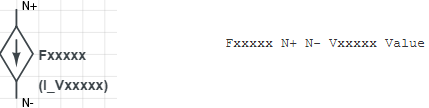
\includegraphics[]{F.png}
	\caption{Netlist format describing a CCCS \cite{MNA}}
\end{figure} 
Like the CCVS, this component is controlled by the current through the listed voltage source. It is handled similarly like CCVS.
CCCS creates one more unknown variable.
\begin{figure} [h!]
	\centering
	\begin{subfigure}{.5\textwidth}
	  \centering
	  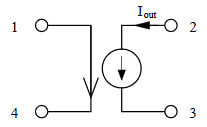
\includegraphics[scale=0.8]{F_diagram.PNG}
	  \caption{Circuit symbol of a CCCS}
	  \label{fig:sub1}
	\end{subfigure}%
	\begin{subfigure}{.5\textwidth}
	  \centering
	  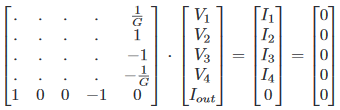
\includegraphics[width= \textwidth]{F_matrices.PNG}
	  \caption{MNA matrix entry}
	  \label{fig:sub2}
	\end{subfigure}
	\caption{MNA matrix for a CCCS \cite{jahn_margraf_habchi_jacob_2003}}
	\label{fig:test}
\end{figure}


\pagebreak
\section{Reflections}
\subsection{Xin Wang}
The project has made me realise that engineering is not only about the practical aspects that many see engineering as. 
Engineering requires as much work, if not more, in planning and documentation than implementing the ideas. 
\par
Through serving as the person in charge of documentation and project management, I have gained an appreciation for the 
work that goes on the background and the role has challenged me to gain new skills such as learning how to write 
Latex documents and researching how a project team can be efficiently managed. 
\par 
I was initially worried that I would not be able to understand the program designs and be relegated to just being a 
minute keeper but, actually, my role required me researching the theory required to implement the program designs and it made 
realise that each role in the team is equally as important and it is important that the team communication effectively and 
be able to work together. As it is our first time handling a project like this, time was wasted with trial and error to work 
out a suitable team dynamic and, with COVID-19, we had to manage this is a remote working environment. It was frustrating but 
the skills gained are unquestionable.
\par 
Due to the repatriation flight, the project had an element of family obligations in it which made it 
more realistic for me. The workplace is not just about working and sometimes family emergencies require you to balance the 
two sides of your life. It is my view that, though the program might not have been realised to its full potential, the 
teamwork and management lessons I learnt made it all worth it and it has inspired me to read more about project management to 
allow me to contribute more the next time I work in a team. 

\subsection{Brandon Cann}
I believe that this project was the first step into the engineering industry where it required us as a team to combine our 
strengths to complete an objective. This project helped me realise the importance of communication and time efficiency. 
\par
My main role of the team was to make sure that each member of the team was updated on each other’s progress and to complete 
any areas where a member had fallen behind or could not complete. 
\par
At the start of the project, the communication between the team was not particularly great where we had two members working 
on the exact same part of the code which was a huge waste of time. Soon after this realisation we organised a team meeting 
to clear up the uncertainties and from there on were on a more efficient path towards completion. Being the only member of 
the team that knew both team members well enough really helped me act as the centre of communication for the team. 
\par
As there was a team member with an emergency to attend to, we were left as two. This meant that I was now responsible to 
make sure both of us were aware of what was left to be completed and to distribute the workload between us. This was a great 
addition to my skill set as I am not usually comfortable with being in a lead role but being forced into this situation 
helped to make quick decisions on the way forward. I hope that the skills learned help me to deal with situations that are 
unforeseeable and make me an invaluable team member. 

\subsection{Adam Rehman}

\pagebreak
\section{Appendix}
\subsection{Belbin Roles}
\begin{figure} [h!]
	\centering
	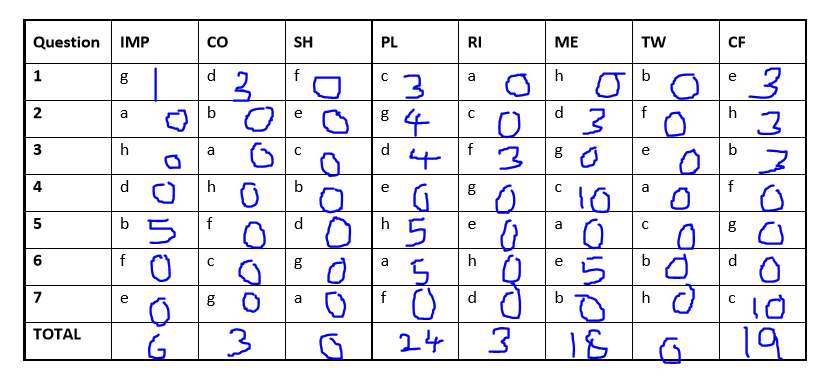
\includegraphics[scale=0.5]{Adam.PNG}
	\caption{Belbin Roles of Adam Rehman}
\end{figure}
\begin{figure} [h!]
	\centering
	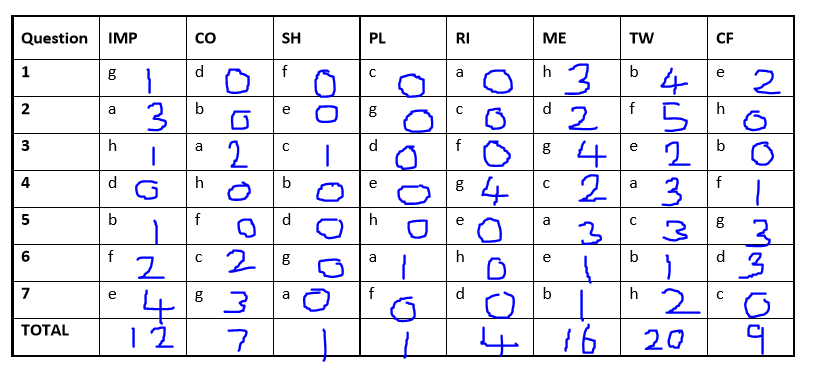
\includegraphics[scale=0.5]{Brandon.PNG}
	\caption{Belbin Roles of Brandon Cann}
\end{figure}
\begin{figure} [h!]
	\centering
	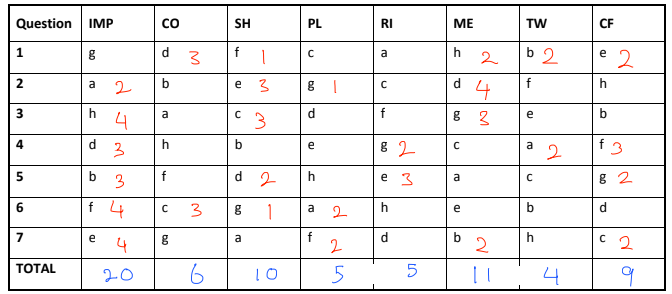
\includegraphics[scale=0.75]{Xin.PNG}
	\caption{Belbin Roles of Xin Wang}
\end{figure}
\pagebreak

\begin{landscape}
	\subsection{Gnatt Chart}
	\begin{center}
		\begin{figure}[htb]
		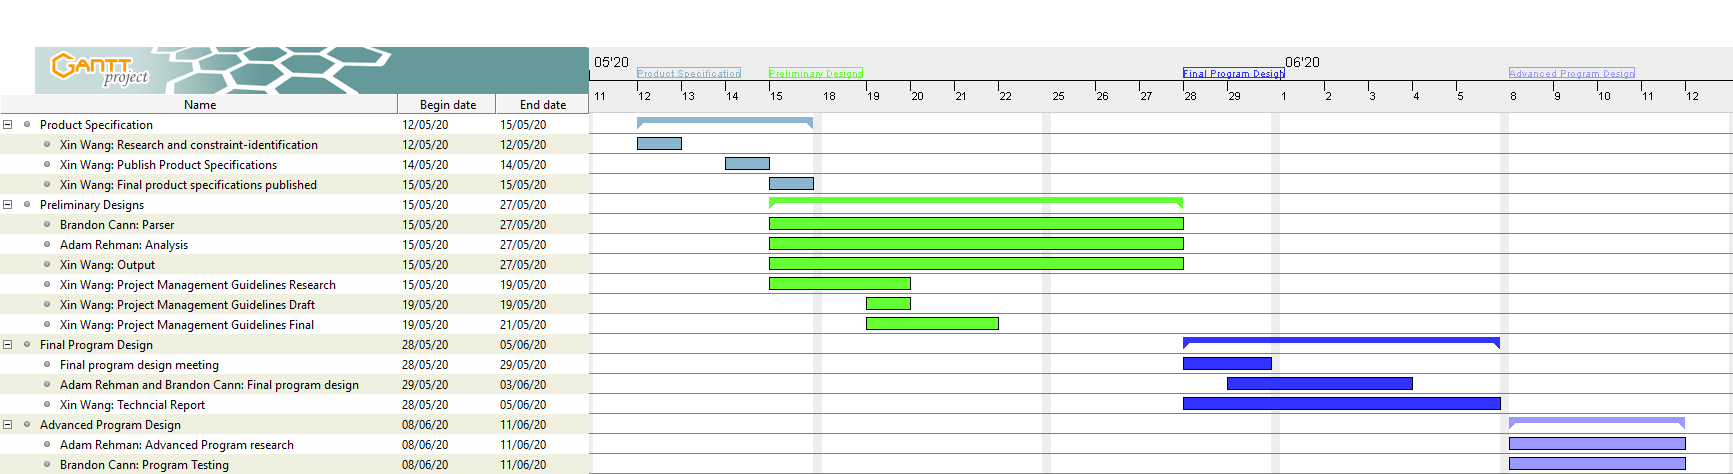
\includegraphics[width=\linewidth]{Project Gnatt.PNG}
		\caption{Gnatt Chart of Team Project}
		\label{fig:landscape}
		\end{figure}
	\end{center}
\end{landscape}
\pagebreak

\subsection{Meeting Minute Template}
\begin{figure}[h!]
	\centering
	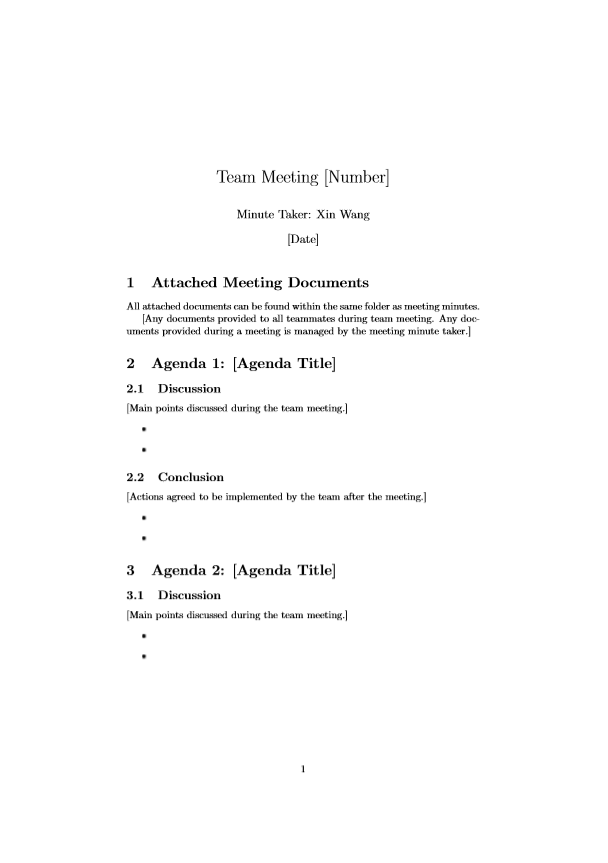
\includegraphics[width=\textwidth]{Minute1.PNG}
\end{figure}

\begin{figure}[h!]
	\centering
	
\includegraphics[width=\textwidth]{Minute2.PNG}
\end{figure}
\pagebreak

\section{References}
\printbibliography
\end{document}